\chapter{Background\label{cha:chapter2}}
As the main objective of this thesis is to develop a framework that manages the correlation between the content and its context and also to provide an efficient and scaleable discovery and distribution mechanism, this chapter gives an overview of the context and how it can be described in order to efficiently use these context data. Furthermore, this chapter deals with related technologies, which could be a part of the developed framework.

\section{Context-awareness\label{sec:back_con_aw}}
In this section, the terms \textit{context} and \textit{context-aware computing} are discussed in more detail. Furthermore, the application possibilities of context awareness is demonstrated.

In order for computers to assist users in their everyday tasks, they should adapt themselves to the current user's situation, and then respond according to this. 

Humans are quite successful at conveying ideas to each other and reacting appropriately. This is due to many factors including the richness of the language they use, the common understanding of how the world works, and an implicit understanding of every-day situations. When humans talk with each other, they are able to use implicit situational information, or context, to increase the conversational bandwidth. Unfortunately, this ability to convey ideas does not transfer well to humans interacting with computers \cite{Dey2000b}.

\subsection{What is Context?}

The report that first introduces the term \emph{context-aware}, [\citeauthor{ieee313011}] refers to context as location, identities of people and objects nearby, and changes to those objects. A similar definition, [\citeauthor{ieee626984}] describes context as location, identities of the people around the user, the time of day, season, temperature, etc. [\citeauthor{Ryan97}] defines context as the user's location, environment, identity and time. [\citeauthor{Dey98}] enumerates context as the user's emotional state, focus of attention, location and orientation, date and time, objects and people in the user's environment.

A recent definition of context-awareness is described by [\citeauthor{Dey2000b}] who defines it as, context is any information that can be used to characterize the situation of an entity. An entity is a person, place, or object that is considered relevant to the interaction between a user and an application, including the user and the application themselves. 

This way, it is easier for an application developer to enumerate the context for a given application scenario. If a piece of information can be used to characterize the situation of a participant in an interaction, then that information is regarded as context.

After the term \textit{context} has been defined the term \textit{context-aware computing} is discussed in the following subsection.

\subsection{Context-aware Computing}
Context-aware computing was first described by [\citeauthor{ieee313011}] in 1994 to be software, that adapts itself according to the location of use, the collection of nearby people and objects, as well as changes to those objects over time. However, it is commonly agreed, that context-aware computing was first investigated in 1992 by [\citeauthor{WantHFG92}]. 

[\citeauthor{RyanME}] has also defined the term context-aware applications as applications that allow users to select from a range of physical and logical contexts according to their current interests or activities and also monitor input from environmental sensors.

\subsection{Context Examples}
The orientation of the screen of a tablet computer is automatically changed, maps can orientate themselves according to the user's direction with the zoom level adapted to the current speed, and the backlight of the phone is switched on when used in the dark.

These are examples of computers that are aware of their environment and their contextual use. However, such functions were not common 10 years ago and only existed on prototype devices in research labs which researched context-aware computing.
\\

Below are some examples of context awareness in mobile and non-mobile environments. Although non-mobile environments for this thesis are not relevant, they are interesting at this point in order to show the diverse application areas which illustrate the usage context-awareness of systems.

\begin{itemize}
\item identity
\item spatial information\\
e.g. location, orientation, speed and acceleration
\item temporal information\\
e.g. time of the day, date and season of the year
\item environmental information\\
e.g. temperature, air quality and light or noise level
\item social situation\\
e.g. who you are with, and people nearby
\item resources that are nearby\\
e.g. accessible devices, and hosts
\item availability of resources\\
e.g. battery, display, network and bandwidth
\item physiological measurements\\
e.g. blood pressure, heart rate, respiration rate, muscle activity and tone of voice
\item activity\\
e.g. talking, reading, walking and running
\end{itemize}

\section{Context Description\label{sec:back_con_de}}
In order to efficiently use the context data after acquisition, it needs to be represented and/or stored in an appropriate form suitable for further processing. Now some of the different types of context modeling will be discussed.

\begin{itemize}
\item \textbf{Key-value model:}  This modeling technique represents contextual information with key-value pairs which is one of the most simple data structures for modeling contextual information. This model was already used in 1994 by \citeauthor{ieee512740} to present the context by providing the value of context information (e.g. location information) to an application as an environment variable. Distributed service frameworks  frequently use the key-value modeling approach. Although key-value pairs lack the capability for sophisticated structuring to enable efficient context retrieval algorithms, they are easy to manage.

\item \textbf{Logic based model: } Logic-based models have a high degree of formality. Typically, facts, expressions and rules are used to define a context model \cite{BaldaufDustdarRosenberg07ijahuc}.

A logic based model defines the conditions on which a concluding expression or fact may be derived (a process known as reasoning or inferencing) from a set of other expressions or facts. In order to describe these conditions in a set of rules, a formal system is applied. In a logic based context model, the context is consequently defined as facts, expressions and rules. Usually contextual information is added to, updated or deleted from a logic based system in terms of facts or inferred from the rules in the system respectively. A high degree of formality is common to all logic based models \cite{Strang2004}.

In early 1993 \citeauthor{McCarthy1993Notes} and his group at Stanford University researched one of the first logic based context modeling approaches and published it as a \textit{Notes on formalizing contexts}. They introduced contexts such as abstract mathematical entities with properties which are useful in artificial intelligence.


\item \textbf{Ontology based model: }
Ontologies are promising instruments to specify concepts and interrelations \cite{gruber_1993}. The \ac{OWL} is one way of implementing these ontologies. This consists of a set of classes, class hierarchies, a set of property assertions, constraints on these elements and types of permitted relationships between them. Another way to implement the ontologies, is to use knowledge representation language - the \ac{RDF}. This is a promising model because of the possibility of applying reasoning techniques \cite{Riva04}.  

\citeauthor{Oeztuerk97towardsa} proposed one of the first approaches of modeling the context with ontologies. Psychological studies on the difference between recall and recognition of several issues in combination with contextual information were analyzed by them. The necessity of normalizing and combining the knowledge from different domains was derived from this examination. A context model based on ontologies due to their strengths in the field of normalization and formality was proposed by them.

\item \textbf{Graphical models:} 
The \ac{UML} is a wide spread modeling tool for software systems. When using \ac{UML}, the architectural aspects of software systems are defined as classes. Each class constitutes a set of objects with common services, properties and behavior. Services are described by methods and properties are described by attributes and associations \cite{Sheng2005}.

\item \textbf{Object-oriented models:} Object-oriented design of context benefits from common properties object-oriented programming, such as inheritance, encapsulation, reuse, and polymorphism. For example, in a model of a payroll system, a company is an object, an employee is another object and employment is a relationship or association. An employee class (or object for simplicity) has attributes like name, birthdate, etc. The association itself may be considered as an object, having attributes, or qualifiers such as position, etc\cite{pSkills:Object-oriented_modeling}.

\item \textbf{Markup languages: } All markup scheme modeling approaches share a hierarchical data structure consisting of markup tags with attributes and content. In particular, the content of the markup tags is usually recursively defined by other markup tags. Typical representatives of this kind of context modeling approach are profiles. They are usually based on a serialization of a derivative of \ac{SGML}, the superclass of all markup languages such as the popular \ac{XML}\cite{Strang2004}.

\end{itemize}

\section{Related Technologies\label{sec:back_rel_tech}}
This section covers a wide of technologies which are relevant for this thesis.	

\subsection{Web Services\label{sec:back_tech_ws}}

There are many definitions for the term Web service, the \ac{W3C} defines it as follows:\cite{W3C}\\
\begin{quote}
A Web service is a software system designed to support interoperable machine-to-machine interaction over a network. It has an interface described in a machine-processable format (specifically \ac{WSDL}). Other systems interact with the Web service in a manner prescribed by its description using \ac{SOAP} messages, typically conveyed using \ac{HTTP} with an \ac{XML} serialization in conjunction with other Web-related standards.
\end{quote}

The \ac{W3C} also states:\cite{W3C} 
\begin{quote}
We can identify two major classes of Web services, \ac{REST}-compliant Web services, in which the primary purpose of the service is to manipulate \ac{XML} representations of Web resources using a uniform set of "stateless" operations; and arbitrary Web services, in which the service may expose an arbitrary set of operations.
\end{quote}

By using Web Services, it is now very easy to make existing data and functions from existing applications available to consumers. Web services are considered as machine to machine communication, which  exchange messages via standard protocols.

The best known web services technologies \ac{SOAP} and \ac{REST} are discussed in the following subsections.

\subsubsection{SOAP\label{sec:back_tech_ws_soap}}
\ac{SOAP} stands for "Simple Object Access Protocol" and it relies on  \ac{XML} for its message format. For message negotiation and transmission, it is dependent on other Application Layer protocols, particularly on \ac{HTTP} or  \ac{SMTP}, however \ac{HTTP} has gained a wider acceptance, as it works well with today's Internet infrastructure and also with network firewalls.

A \ac{SOAP} message is a type of envelope or container, which may contain an optional header element and a mandatory body element, see figure \ref{fig:soap_env}. Meta-data for this message are located in the header and the user data are stored in the body.

\begin{figure}[htb]
  \centering
  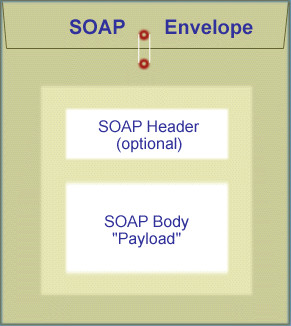
\includegraphics[scale=0.5]{soap_envelope.jpg}\\
  \caption{\ac{SOAP} Envelop}
  \label{fig:soap_env}
  \protect\cite{oracle_soap}
\end{figure}

\paragraph{\ac{SOAP} Message Example:}

Listing \ref{lst:soap_message} is an example, which gives an overview of a \ac{SOAP} message:

\begin{code}
\begin{minted}[frame=single,tabsize=2,fontsize=\footnotesize]{xml}
<?xml version="1.0"?>
<soap:Envelope xmlns:soap="http://www.w3.org/2003/05/soap-envelope">
  <soap:Header>
  </soap:Header>
  <soap:Body>
    <m:GetStockPrice xmlns:m="http://www.example.org/stock">
      <m:StockName>IBM</m:StockName>
    </m:GetStockPrice>
  </soap:Body>
</soap:Envelope>
\end{minted}
\caption{\ac{SOAP} message example}
\label{lst:soap_message}
\end{code}

\subsubsection{\ac{REST}\label{sec:back_tech_ws_rest}}
In addition to \ac{SOAP}, there is another alternative for the implementation of Web services. \citeauthor{Fielding2000} in his dissertation describes an architectural style that he calls REpresentational State Transfer architecture or short \ac{REST}.

\ac{REST} is based on principles that are used in the largest distributed application - the World Wide Web. The World Wide Web is itself a gigantic \ac{REST} application. Many search engines, shops or booking systems have unintentionally been based on \ac{REST} web services.

The REpresentational State Transfer Architecture is an architectural model, which describes how the Web should work. The model will serve as a guide and reference for future enhancements. \ac{REST} is not a product or standard. \ac{REST} describes how web standards in a Web-friendly manner can be used.


\paragraph{REST Example:} An online store will serve here as an example of a RESTful application. In this application, there are customers who can place items in shopping carts.

Each object of the application, such as the product or the customer is a resource that is externally accessible via a \ac{URL}. With the following request in the example application, the shopping cart with the number 7621 is retrieved.

%\lstset{language=JSON}
\begin{code}
\begin{minted}[frame=single,tabsize=2,fontsize=\footnotesize]{console}
GET /cart/7621
\end{minted}
%\caption{Sample configuration file for locations within NginX}
%\label{lst:locations_nginx}
\end{code}


It is not specified in \ac{REST} how the result of a request is represented. Client and server must have a shared understanding how the data is represented, i.e. in \ac{XML} or \ac{JSON}. Listing \ref{lst:json_response} is a response example in \ac{JSON} format.

\begin{code}
\begin{minted}[frame=single,tabsize=2,fontsize=\footnotesize]{json}
{
"customer": 7621,
"articles":[
	{"position":1,
	"articleNumber":89,
	"description":"iPhone5",
	"price":200},
	{"position":2,
	"articleNumber":76,
	"description":"Samsung Galaxy S III",
	"price":150}
	]
}
\end{minted}
\caption{\ac{JSON} response example}
\label{lst:json_response}
\end{code}

\subsubsection{SOAP vs. REST\label{sec:back_soap_vs_rest}}

The main advantages of \ac{REST} web services are that they are lightweight, without a lot of extra \ac{XML} markup. As well \ac{REST} has easy to read results and is easy to build, requiring no special tool-kits.

\ac{SOAP} also has some advantages. Usually it is easy to use, provides relatively strong typing, since it has a fixed set of supported data types and as well, many different kinds of development tools are available.

Next some aspects of \ac{SOAP} and \ac{REST} will be compared.

\paragraph{API Flexibility \& Simplicity}

The key to the \ac{REST} methodology is to use an interface that is already well known and widely used, the \ac{URI}, in order to write web services. For example, providing a currency converter service, in which a user types-in the desired currencies for input and output and the specific amount in order to receive a real-time conversion, could be as simple as making a script accessible on a web server via the following \ac{URI}: http://www.currencyconverter.com/convert?in=us-dollar\&value=100\&out=euro

This service could easily be requested with an \ac{HTTP} GET command by any client or server application with \ac{HTTP} support. The resulting \ac{HTTP} response depends on how the service provider wrote the script and it might be as simple as some standard headers and a text string containing the current price for the given currencies, or it might be an \ac{XML} document.
\\
\\
The significant advantages of this interface method over \ac{SOAP}-based services are as follows:-
\\
\\
The creation and modification of a \ac{URI} in order to access different web resources can easily be figured out by any developer. However, in order for \ac{SOAP} to be used, most developers would need a \ac{SOAP} toolkit to form requests and obtain the results, as it requires specific knowledge of a new \ac{XML} specification.
\\
\\
\paragraph{Bandwidth Usage}

The RESTful interface has short requests and responses, which is another advantage, whereas, an \ac{XML} wrapper around every request and response is required for \ac{SOAP}. For a four- or five-digit stock quote, a \ac{SOAP} response may require more than 10 times the number of bytes for the same response in \ac{REST}, as \ac{SOAP} requires namespaces and typing to be present. 
\\
\\
\paragraph{Security}
The security perspective debate is probably the most interesting aspect of the comparison between \ac{REST} and \ac{SOAP}. 

Sending \ac{RPC} through standard \ac{HTTP} ports is seen by the \ac{SOAP} camp as being a good way to ensure Web services support across organizational boundaries. In contrast however, \ac{REST} followers see this as compromising network safety and considers this practice a major design flaw.

With \ac{REST}, the administrator (or firewall) can discern the intent of each message by analyzing the \ac{HTTP} command used in the request, even though the \ac{REST} calls also go over \ac{HTTP} or \ac{HTTPS}. For example, a GET request is always seen as being safe, because by definition, the data cannot be modified, it can only query data.

On the other hand, \ac{HTTP} POST is used by a typical \ac{SOAP} request to communicate with a given service. Without looking into the \ac{SOAP} envelope, it is not possible to know whether the request simply wants to query data or delete entire tables from the database. This task is resource-consuming and it is not built into most firewalls.

On the downside, with \ac{SOAP}, the difficult task of authentication and authorization is left up to the application developer. However, the fact that the web servers already have support for these tasks is taken into account by the \ac{REST} methodology. \ac{REST} methodology developers can make the network layer do all the heavy work by using industry-standard certificates and a common identity management system, such as an \ac{LDAP} server.

However, \ac{REST} is not perfect. It is not always the best solution for all web services. Data should never be sent as parameters in \ac{URI}s in order to be kept secure. 

\paragraph{Type Handling}

Due to its fixed set of supported data types, \ac{SOAP} provides stronger typing. In this way, it ensures that a return value  will be given in the corresponding native type in a specific platform. For example, when an \ac{API} is \ac{HTTP} based, the return value will need to be deserialized from its original \ac{XML} format before being type-casted.    
However, handling complex data-types proves to be the main challenge and is mainly achieved by defining a serialization and deserialization mechanism, therefore, there ease of client-side coding has no definitive advantage. 


\paragraph{Client-side Complexity}

Making calls to an \ac{REST} \ac{API} poses less of a challenge than making calls to a \ac{SOAP} \ac{API}. While \ac{REST} is elementary to all programming languages and merely implies constructing an \ac{HTTP} request with the appropriate parameters, the latter requires a client library, a Stub and involves additional learning.  

\paragraph{Testing and Troubleshooting}

A further characteristic of \ac{REST} \ac{API}s is their easy testing and troubleshooting ability, requiring no more than a browser, the response appearing in the browser window itself. Generating a request does not require special test tools which is a major advantage of \ac{REST} based \ac{API}s.  
  

\paragraph{Server-side Complexity}

The majority of programming languages provide easy to operate mechanisms in order to expose a method using \ac{SOAP}. However, exposing a method using \ac{REST} based \ac{API}s involves additional effort due to the task of mapping the \ac{URI} path to specific handlers. Though various frameworks facilitate this task, the exposition of methods is still easier to achieve using \ac{SOAP} than \ac{REST}.

\paragraph{Caching}

To consume a \ac{REST} based \ac{API} service, a simple GET request is needed, therewith allowing proxy servers to cache their response very easily. In contrast, \ac{SOAP} requests use POST and requires a complex \ac{XML} format, producing difficulties for response-caching.

\subsection{NoSQL Databases \label{sec:back_da_per}}
\ac{SQL} databases have been used to solve storage problems for a long time, including cases in which there is a high discrepancy between the object model and its relational model. The conversion of graphs to tables represents yet another dis-functional use of data mapping. The complex structure of these kinds of mismanagement causes, depends on mapping frameworks and complex algorithms. The rigid relational scheme characteristic for \ac{SQL} becomes especially inefficient for such web applications as blogs, due to their multifaceted range of attributes that need to be stored in their respective tables, e.g. comments, pictures, audios, videos and source codes. Therefore, adding or removing a new feature to this sort of website could result in system unavailability.          

Nowadays of course,  web sites are developing towards more interactive models, obliging databases to perform real-time schema updates, thereby paving the way for \ac{NoSQL} to provide a database molded for modern demands.

There are a variety of ideas surrounding the \ac{NoSQL} movement, however, the core idea is to provide more flexible data models, as opposed to the \ac{SQL} approach, in order to provide live schema updates. The ever increasing amount of data streaming through the web implies challenges, which any competitive website wishing to stay in business will have to meet. Besides dealing with vast amounts of data, these sites have to respond to constant requests around the globe without allowing any noticeable latency.

To this end, many companies have developed their own storage systems, according to their specific needs, which have been classified as \ac{NoSQL} databases. Considering the fact that these stores are set up to fulfill the individualized requirements of the companies they belong to, there can be no final answer as to which one works most efficiently. For example, Facebook implemented the \ac{NoSQL} database Cassandra, in order to solve the so called "Inbox Search Problem" - the challenge of allowing Facebook users to search through their sent and received messages - caused by the multitude of stored data along with the high number of active users. 
\\
\\
A selection of the most known \ac{NoSQL} systems are shown in Table \ref{tbl:nosql_sys}, which are categorized into the following groups: Key Value Stores, Document Stores, Column Family Stores and  Graph Databases
\\
\\
\begin{table}[htb]
\begin{tabular}{|c|c|c|c|}
\hline 
\textbf{Key Value Stores} & \textbf{Document Stores} & \textbf{Column Stores} & \textbf{Graph Databases} \\ 
\hline 
$\begin{array}{l} \textbf{Riak} \\ \textbf{Amazon SimpleDB} \\ \textbf{Voldemort}\\  \textbf{Redis} \end{array}$ & 
$\begin{array}{l} \textbf{CouchDB} \\ \textbf{MongoDB} \\ \textbf{Couchbase} \end{array}$ & 
$\begin{array}{l} \textbf{HBase} \\ \textbf{Hypertable} \\ \textbf{Cassandra}  \end{array}$  & 
$\begin{array}{l} \textbf{Neo4J} \\ \textbf{AllegroGraph}   \end{array}$ \\ 
\hline 
\end{tabular}
\caption{Most known NoSQL systems}
\label{tbl:nosql_sys}
\end{table}
\\
\\

The following subsections will examine these groups, each accompanied by one or more exemplary implementations.      

\subsubsection{Key Value Stores}

Key value stores provide suitable storage systems for simple operations, based on key attributes only. They can be compared to maps or dictionaries due to the fact that data is identified by a unique key. They allow for a user specific webpage to be partially calculated beforehand and consequently be served quickly to the user when requested. Most key value stores save their data in memory, so they are frequently used for the caching of more time intensive \ac{SQL} queries. Examples for key value stores are Project Voldemort, Redis, Membase and Riak and the latter will be described in detail in the following paragraph.

\paragraph{Riak:} Riak is a distributed, scalable, open source key/value store. Riak scales predictably and easily and simplifies development by giving users the ability to quickly prototype, test, and deploy their applications. One of two ways to access data in Riak is by using a \ac{REST} \ac{API}. The other way to access data is through a fully-featured Protocol Buffers \ac{API}. This is a simple binary protocol based on the library Google's open source project of the same name.

The only one way to organize data inside of Riak is by using buckets and keys. Data is stored and referenced by bucket/key pairs. These buckets are used to define a virtual keyspace and provide the ability to define isolated non-default configuration. They might be compared to tables or folders in relational databases or file systems respectively \cite{Riak:Buckets}.

Interactions with Riak are either setting or retrieving the value of a key. The following describes this using the Riak \ac{HTTP} \ac{API}. In order to read an object, a basic request is used to retrieve a specific key from a bucket. 

\begin{code}
\begin{minted}[frame=single]{console}
GET /riak/bucket/key
\end{minted}
%\caption{My Func}
\label{lst:riak_get}
\end{code}

The body of the response will contain the content of the object (if it exists).
\\
\\
For storing an object with a user-defined key, the basic request looks like this:

\begin{code}
\begin{minted}[frame=single]{console}
PUT /riak/bucket/key
\end{minted}
%\caption{My Func}
\label{lst:riak_get}
\end{code}

There is no need to explicitly create a bucket because it is automatically created when keys are added to them.


\subsubsection{Document Stores}
Document Stores interlace key value pairs in \ac{JSON} or \ac{JSON} like documents. Each of these documents contains a special key \textit{ID}, which is unique throughout a collection of documents and therefore identifies a document explicitly. 

Key value stores don't allow values to be queried, because the values are only accessible through their respective keys. Document stores on the other hand, provide mechanisms for this additional function. They therefore allow complex data structures to be handled more efficiently. The interpretable \ac{JSON} format applied by document stores ensures a developer frien	dly usage by supporting data types. In contrast to key value stores which focus on high performance for read and write concurrent, document stores concentrate on storing big data efficiently while also providing high query performance. The most known document stores are CouchDB and MongoDB  which are described in detail in the following paragraphs.

\paragraph{CouchDB:} CouchDB is a free open source document oriented database developed by Apache Software Foundation. It is written in Erlang, a programming language aimed at concurrent and distributed applications. It was first released in 2005 and in 2008 it became an Apache project.

CouchDB implements a \ac{MVCC} to avoid the need to lock the database file while writing. The application has to be aware of resolving conflicts, which generally involves merging data into one of the documents, then deleting the stale one.

CouchDB adopts a semi structured data model based on \ac{JSON} format, which is a collection of named key-value pairs. The value can either be a number, string, boolean, list or a dictionary. The data model is completely schema-free and it only needs to be conformed to the \ac{JSON} specification. An example document is shown in listing \ref{lst:couch_doc}, which represent the apple price in various supermarkets. 
\\
\\
\begin{code}
\begin{minted}[frame=single]{json}
{
    "_id" : "bc2a98726578c326ec68382f846d7629",
    "_rev" : "8763642898",
    "item" : "apple",
    "prices" : {
        "ALDI" : 1.59,
        "LIDL" : 5.99,
        "Kaufland" : 0.79
    }
}
\end{minted}
\caption{Example of a CouchDB document}
\label{lst:couch_doc}
\end{code}

Each document is identified by a unique ID (the \textit{id} field) within a CouchDB database . CouchDB can simply be seen as a collection of documents and it does not know or track relationships between documents \cite{books:daglib:0024051}.  It provides a RESTful \ac{HTTP} \ac{API} to perform basic CRUD operations on all stored documents, which can easily be done via the \ac{HTTP} methods POST, GET, PUT and DELETE.

Figure \ref{fig:couchdb_repl} illustrates how easy the data synchronization is between any two databases. After replication, each database is able to work independently.

\begin{figure}[htb]
  \centering
  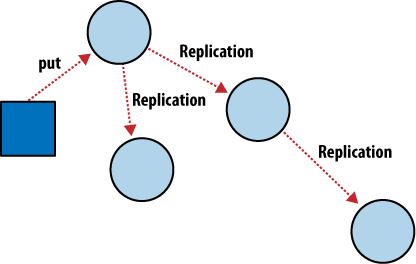
\includegraphics{couchdb_repl.png}\\
  \caption{CouchDB replication}
  \label{fig:couchdb_repl}
  \protect\cite{couchdb_cons}
\end{figure}

CouchDB relies on the \ac{MVCC} model for handling conflicts. Each document has a revision id and on each update of a document, the old version is kept and the new version is given a different revision id. In case of a conflict, the desired version is always saved as the most recent version and the old version is saved in the document's history. Thereby, the application handles the conflict by itself and decides which version is the desired one to keep and which is the old one \cite{books:daglib:0024051}.

\paragraph{MongoDB:\label{sec:back_mongo}}
MongoDB is a free and open source document oriented database written in C++ that provides high performance, high availability, and easy scalability. The development is supported by the open source community and also by the company 10gen. As in CouchDB, it is completely schema-free and its data model is based on \ac{JSON} format  that is easy to code, easy to manage, and yields excellent performance by grouping relevant data together internally \cite{mongodb_intro}. 

The document structure in MongoDB are BSON objects, short for Binary \ac{JSON}, which is a binary-encoded serialization of \ac{JSON}-like documents.  \ac{BSON} supports all \ac{JSON} data types but also defines new types, i.e. the Date data type and the BinData type \cite{bson_intro}.

Like CouchDB, the documents are saved within collections, which can be compared to tables in relational databases. All kinds of documents can be stored within collections but in order to provide a logical way of organizing data, the documents within a collection usually have the same structure.

MongoDB provides two ways for replication, namely Replica Sets and Master-Slave, see figure \ref{fig:mongodb_repl}. Master-Slave replication has been deprecated since version 1.6 therefore Replica Sets are used for all new production deployments.

\begin{figure}[htb]
  \centering
  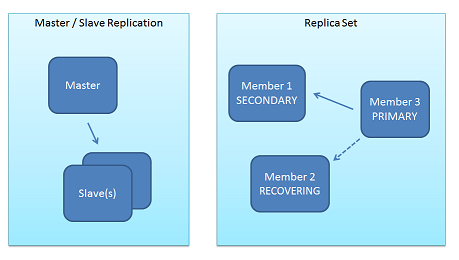
\includegraphics{mongodb_repl.png}\\
  \caption{MongoDB replication}
  \label{fig:mongodb_repl}
  \protect\cite{mongodb_replication}
\end{figure}

\subsubsection{Column Stores}
Column Family Stores are known as column oriented stores, extensible record stores or wide columnar stores. All stores are inspired by Googles Bigtable, which is a distributed storage system for managing structured data that is designed to scale to a very large size.\cite{Hecht:2011,Chang:2006} 

Bigtable has been used by Google in many projects, which require high throughput and low latency data serving. The data model is described as a sparse, distributed, persistent multidimensional sorted map \cite{Chang:2006} . Any number of key value pairs can be stored in rows within a map. In contrast to document stores, column stores cannot be queried by value and therefore one is required to write the data the way one intends to read it, meaning one must think about the data model in terms of ones queries. In order to achieve both versioning and consistency, multiple versions of a value are stored chronologically. 

Big companies such as Google and Facebook, use their respective Column Family Stores (BigTable and Cassandra) to store data in the same way, as it will be required when requested later on. This sort of storage  ensures that only one data retrieval is needed when a request is launched, therefore saving considerable effort and maximizing performance as compared to the conventional process via MySQL which often requires multiple queries.  

\paragraph{Cassandra:}
Apache Cassandra is a free and open source distributed, structured key-value store with eventual consistency. It was initially developed by Facebook and now is developed by the Apache Foundation. It is designed to handle very large amounts of data, while providing high availability and scalability.

A table in Cassandra is a distributed multi dimensional map indexed by a key. The value is an object which is highly structured \cite{biba2011learning}. Columns are grouped together into sets called column families very similar to the Bigtable system. Cassandra exposes two kinds of these columns families, Simple and Super column families. Super column families can be visualized as a column family within a column family\cite{biba2011learning}.

Furthermore, applications can specify the sort order of columns within a Super Column or Simple Column family. The system allows columns to be sorted either by time or name. Time sorting of columns is exploited by the application Inbox Search where the results are always displayed in time sorted order.

\citeauthor{Lakshman:2010} have introduced in their article \cite{Lakshman:2010} the Facebook Inbox Search in which they maintain a per user index of all messages that have been exchanged between the sender and the recipients of the message. They introduced two kinds of search features, namely \textit{term search} and \textit{interactions} - given the name of a person returning all messages that the user might have ever sent or received from that person. The schema consists of two column families. For query a \textit{term search}, the user id is the key and the words that make up the message become the super column. Individual message identifiers of the messages that contain the word become the columns within the super column. For a query an \textit{interactions} again the user id is the key and the recipients id's are the super columns. For each of these super columns the individual message identifiers are the columns. In order to make the searches faster, Cassandra provides certain hooks for intelligent caching of data. For instance, when a user clicks into the search bar, an asynchronous message is sent to the Cassandra cluster to prime the buffer cache with that user's index. This way, when the actual search query is executed, the search results are likely to already be in memory. The system currently stores about 50+TB of data on a 150 node cluster, which is spread out between east and west coast data centers. Table \ref{tbl:nosql_cas} shows some production measurement for read performance.

\begin{table}[htb]
\begin{tabular}{|c|c|c|}
\hline 
Latency Stat & Search Interactions & Term Search \\ 
\hline 
Min & 7.69ms & 7.78ms \\ 
\hline 
Median & 15.69ms & 18.27ms \\ 
\hline 
Max & 26.13ms & 44.41ms \\ 
\hline 
\end{tabular} 
\caption{Cassandra production measurement for read performance by Facebook}
\label{tbl:nosql_cas}
\protect\cite{Lakshman:2010}
\end{table}

\subsubsection{Graph Databases}
Graph databases are specialized with efficient management of heavily linked data and therefore are more suitable for applications based on data with many relationships, thereby cost intensive operations such as recursive joins can be replaced by efficient traversals \cite{Hecht:2011}.

Neo4j and GraphDB are examples of graph databases. They are based on directed and multi relational property graphs. Nodes and edges consist of objects with embedded key value pairs. The range of keys and values can be defined in a schema, whereby the expression of more complex constraints can be easily described. Therefore, it is possible to define that a specific edge is only applicable between a certain types of nodes. Use cases for graph databases are location based services, knowledge representation and path finding problems raised in navigation systems, recommendation systems and all other use cases which involve complex relationships \cite{Hecht:2011}.

Twitter has implemented their own graph database FlockDB in which they store a lot of relationships between people in order to provide their tweet following service. These one-way relationships are handled by FlockDB which is optimized for very large adjacency lists, fast reads and writes.

\paragraph{Neo4J:}
Neo4J is an open source project implemented in Java and has been developed by Neo Technology since 2007. In contrast to relational databases, which map nodes and edges in tables, Neo4J supports these graph elements natively which involves an easy structure of the data model.

The node is the basic component within a graph in Neo4J, which has a unique and continuous ID. Nodes can optionally have schema-less properties such as key-value pairs which means that each node can have different keys. This is more flexible than relational databases, which need a separate table for each node type. 

A special node within Neo4J is the reference node or the so-called root node, which is the entry point of each graph. This node is automatically created while creating a new database. Each node should be indirectly connected to the reference node in order to be reachable to the reference node.

The edge is another component of the graph in Neo4J, which connects nodes together and provides a mechanism to traverse over the database tree. Similar to nodes, edges have an unique ID and optional schema-less properties such as key-value pairs.

Neo4J supports two types of deployment, either as embedded or as a server, see figure \ref{fig:neo4j}.

\begin{figure}[htb]
  \centering
  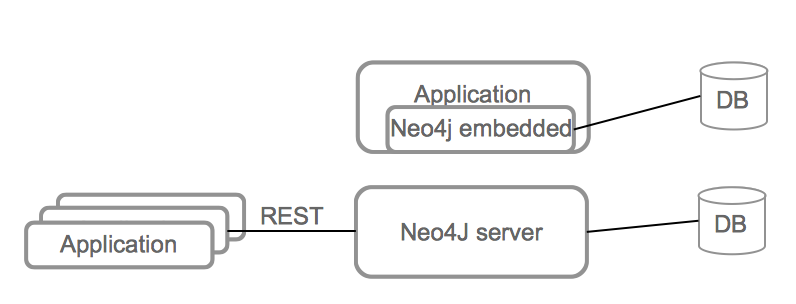
\includegraphics[scale=0.4]{neo4j_n.png}\\
  \caption{Embedded  vs. Server deployment of Neo4J}
  \label{fig:neo4j}
\end{figure}

\subsection{Message broker\label{sec:back_me_mid}}
A Message Broker is a centralized hub that simplifies communication among heterogeneous systems \cite{books/daglib/0013993}. It hosts messaging destinations like queues and topics for the purposes of asynchronous communication, meaning that the sender and receiver of a message do not need to interact with the message queue at the same time. Messages placed in a queue are stored until the recipient retrieves them. There are a number of open source choices of message brokers, including JBoss Messaging, Apache ActiveMQ, WebSphere Message Broker, BizTalk and RabbitMQ.

\paragraph{RabbitMQ}

RabbitMQ is an open source message broker which implements the \ac{AMQP} standard. It has been developed by Rabbit Technologies Ltd. which was acquired in April 2010 by VMWare.

Figure \ref{fig:rabbit_mq} shows the four basic components of the \ac{AMQP} concept which consist of a producer, exchange, queue and a consumer. Producers publish messages to exchanges, which can be compared to post offices or mailboxes. Exchanges then distribute these messages to queues using rules called bindings. Messages are then delivered to consumers subscribed to queues, or the consumers fetch/pull messages from queues on demand \cite{amqp-concepts}.
\begin{figure}[htb]
  \centering
  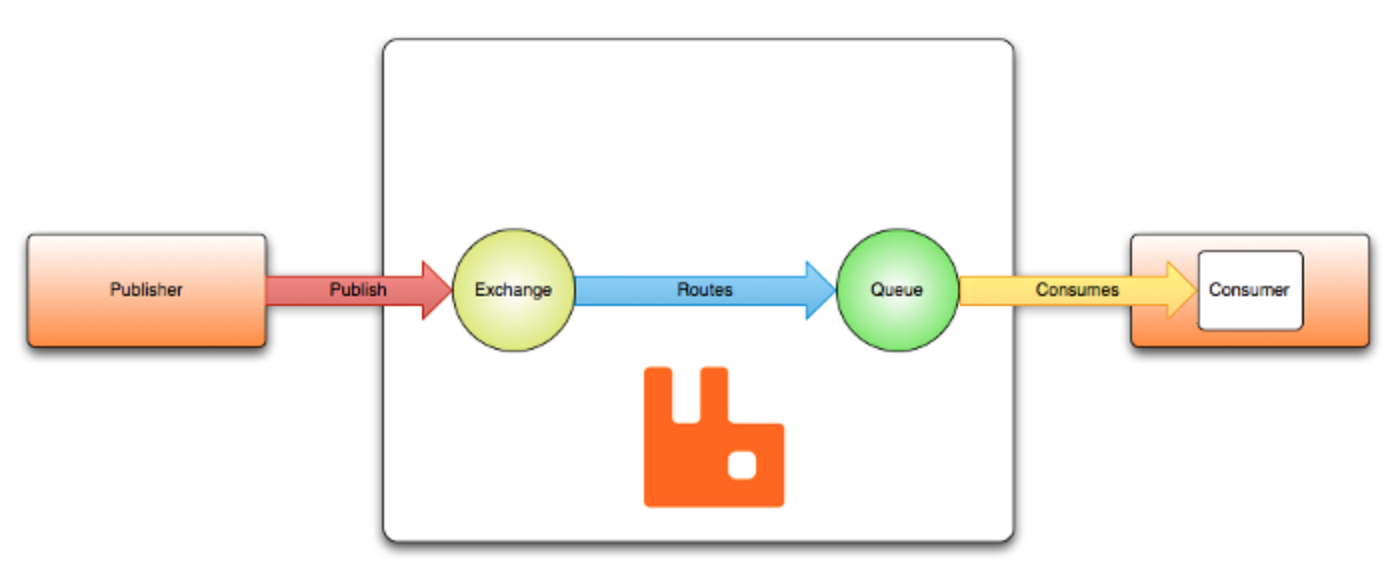
\includegraphics[scale=0.6]{rabbit_mq.png}\\
  \caption{RabbitMQ Components}
  \label{fig:rabbit_mq}
  \protect\cite{amqp-concepts}
\end{figure}

Thereby, the producer never sends the message directly to a message queue, rather to the exchange. Hereby, the exchange must know what to do with the message and to which message queue it should be forwarded to. This is the task of the rules that are defined by four different exchange types:  topic, headers, direct and fanout, the last two types being described below.

\begin{itemize}
\item{\textbf{Direct:}} Direct exchanges are often used to distribute tasks between multiple workers (instances of the same application) in a round robin manner. When doing so, it is important to understand that, in \ac{AMQP} , messages are load balanced between consumers and not between queues \cite{amqp-concepts}, see figure \ref{fig:rabbit_mq_direct} for an illustration.

\begin{figure}[htb]
  \centering
  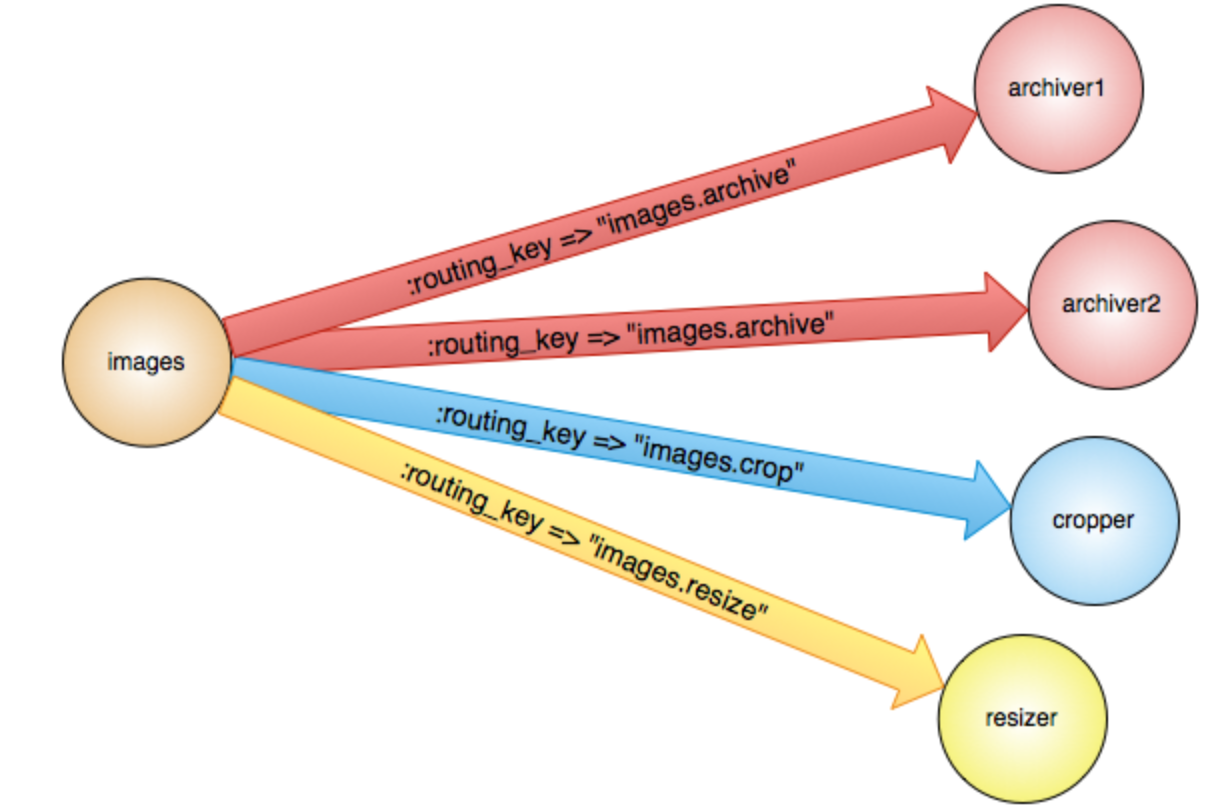
\includegraphics[scale=0.6]{rabbit_mq_direct.png}\\
  \caption{Direct exchange routing}
  \label{fig:rabbit_mq_direct}
  \protect\cite{amqp-concepts}
\end{figure}

\item{\textbf{Fanout:}} Fanout exchange routes messages to all of the queues that are bound to it and the routing key is ignored \cite{amqp-concepts}. A fanout exchange can be represented graphically in figure \ref{fig:rabbit_mq_fanout}.

\begin{figure}[htb]
  \centering
  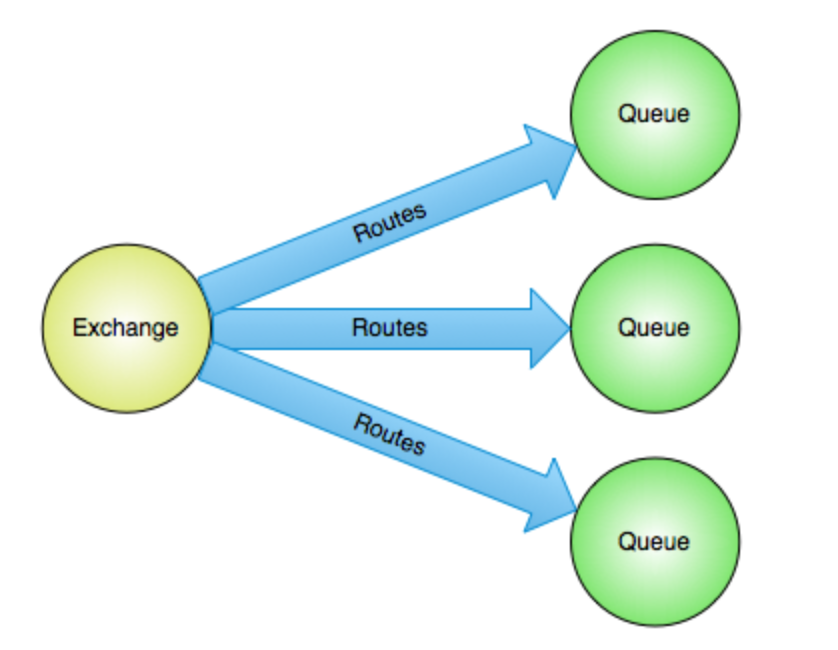
\includegraphics[scale=0.6]{rabbit_mq_fanout.png}\\
  \caption{Fanout exchange routing}
  \label{fig:rabbit_mq_fanout}
  \protect\cite{amqp-concepts}
\end{figure}

\end{itemize}

\paragraph{ActiveMQ}
ActiveMQ is an open source message broker developed by the Apache Foundation and is implemented in Java. ActiveMQ has implemented the Java Message Service (JMS) protocol. The advantage over RabbitMQ is that these brokers can be embedded in a Java application and this simplifies the delivery of a software package. On the other hand, ActiveMQ implemented the \ac{AMQP} protocol first in the version 5.8.0, which was released in February 2013 and therefore their implementation of the \ac{AMQP} protocol have not been widely used or tested in production environments.

\subsection{Search Platforms \label{sec:back_se_en}}
The mean idea behind search engines is to help users to quickly find useful information from the web. There are many available solutions that  perform the task of information retrieval, however, only some of them are popular.

Over time, user queries are becoming more complex and personalized. Where once only a \ac{SQL} LIKE clause was good enough, today's usage sometimes calls for sophisticated algorithms. Fortunately, a number of open source and commercial platforms address the need for more powerful and more widely distributed search technology, including Apache Solr, Amazon's CloudSearch, and Elasticsearch.

\subsubsection{Apache Solr \label{sec:back_se_solr}}

Solr is a popular, blazing fast open source enterprise search platform based on the Apache Lucene project. It is written in Java and runs as a standalone full-text search server within a servlet container such as Tomcat. 

Solr has \ac{REST}-like \ac{HTTP}/\ac{XML} and \ac{JSON} \ac{API}s that make it easy to use from virtually any programming language. Its major features include powerful full-text search, hit highlighting, faceted search, dynamic clustering, database integration, rich document (e.g., Word, PDF) handling, and geospatial search. Solr is highly scalable, providing distributed search and index replication and it powers the search and navigation features of many of the world's largest internet sites \cite{welcome_to_solr}.

\subsubsection{Elasticsearch \label{sec:back_se_es}}

Elasticsearch is an open source search engine implemented in Java and is based on the Apache Lucene project. It provides both an indexing service as well as a data store and does not require a detailed schema. This means that the data which can be expressed as \ac{JSON} can be easily stored and indexed within Elasticsearch. Listing \ref{lst:elasticsearch_schema-free} shows two examples of indexing data that are in \ac{JSON} format. These examples show how easy the schema can be extended, i.e. the second \ac{JSON} data has a new tag called \textit{author}.
 
\begin{code}
\begin{minted}[frame=single]{console}
curl -XPUT http://localhost:9200/blogs/blog/1 -d '{
    "post_date": "2012-12-15T09:00:00",
    "content": "This is the first blog"
}'

curl -XPUT http://localhost:9200/blogs/blog/2 -d '{
    "author": "tom",
    "post_date": "2012-12-16T11:00:00",
    "content": "Second blog"
}'
\end{minted}
\caption{Schema-less Elasticsearch}
\label{lst:elasticsearch_schema-free}
\end{code}


Elasticsearch uses an internal \ac{NoSQL} database system supporting \ac{JSON} documents. Due to its multi-tenancy, an Elasticsearch instance can have more than one index which consists of types, which again consist of fields. Comparable to relational database systems, an index is equivalent to a database, a type is comparable to a table and a field is comparable to a column. No type schema definition is necessary which makes Elasticsearch highly flexible.

One of the unique features of Elasticsearch that makes it especially well suited to distributed systems, is the ease in which it can  can be scaled. It provides the ability to either add or remove resources, which are individual machines running Elasticsearch, at any time in order to support a growing data set or perhaps to satisfy an increasing amount of requests and also improve the performance of the desired solution.

\subsection{Spring Framework\label{sec:back_sp_fr}}
The Spring framework is a lightweight solution and a potential one-stop-shop for building enterprise-ready applications. Due to its modularity, one need only use those parts that one needs, without having to include all other modules i.e. one can use the IoC container, with Struts on top, or else one can use only the Hibernate integration code or the \ac{JDBC} abstraction layer. The Spring Framework supports declarative transaction management, remote access to the application logic through \ac{RMI} or web services, and various options for persisting the data. It offers a full-featured \ac{MVC} framework, and enables integrating \ac{AOP} transparently into  softwares \cite{spring-framework-reference}.


The Spring Framework consists of features organized into about 20 modules. These modules are grouped into Core Container, Data Access/Integration, Web, \ac{AOP}, Instrumentation, and Test \cite{spring-framework-reference}, see figure \ref{fig:spring_arch} for illustration.

\begin{figure}[htb]
  \centering
  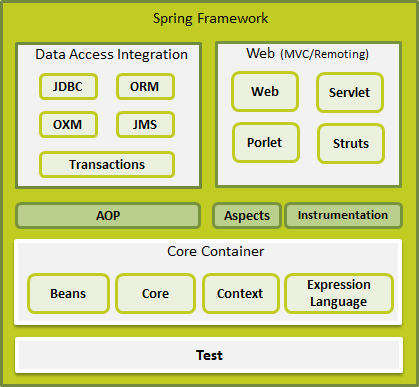
\includegraphics[scale=0.6]{spring_architecture.png}\\
  \caption{Overview of the Spring Framework}
  \label{fig:spring_arch}
  \protect\cite{spring-framework-reference}
\end{figure}